\chapter{RISC-V}
\label{cha:riscv}

\textit{RISC-V} is an open standard Instruction Set Architecture (ISA) based on the
principles of Reduced Instruction Set Computing (RISC). Unlike proprietary ISAs
like \textit{x86} and \textit{ARM}, \textit{RISC-V} is designed to be open and
free, enabling anyone to develop compatible hardware and software without licensing
fees. This openness makes it highly appealing for academia, research, and
commercial applications, as companies can design custom processors tailored to specific
applications while avoiding vendor lock-in.

The \textit{RISC-V} ISA has been defined as an interface to a wide variety of
implementations rather than as the design of a particular hardware. This means that
the same ISA can be used with many processors and is not tailored to a specific one
leaving space for customization, flexibility, and reusability.

In the following sections, we provide a detailed background on the \textit{RISC-V}
ISA and the aspects that are necessary to understand the underlying infrastructure
of the project\footnote{Every information will refer to the $32$-bit \textit{RV32I}
ISA since it is the one utilized in the project.}\footnote{Most of the
information in this chapter is taken from both the Unprivileged and Privileged
Specifications\cite{specifications} published from \textit{RISC-V} International.}.

\section{RISC-V ISA Overview}
\label{sec:riscv_isa}

The \textit{RISC-V} ISA is structured around a minimal base integer ISA, which
is mandatory for all implementations. Even if we refer to the ``base integer ISA''
there are actually four base ISAs within the \textit{RISC-V} family: \textit{RV32I},
\textit{RV64I}, \textit{RV32E}, and \textit{RV64E}, each differing primarily in the
width of integer registers ($32$ or $64$ bits) and the number of available registers
(\textit{E} ISAa support half the number of registers). These variations support
different use cases, from small microcontrollers (\textit{RV32E} and \textit{RV64E})
to larger systems (\textit{RV64I}). Moreover, RISC-V International is currently working
on a $128$-bit ISA known as \textit{RV128I}.

These base ISAs are designed to provide the bare minimum instructions for
essential software tools while allowing for extensive customization and
specialization through additional extensions.

To accommodate customization, \textit{RISC-V} divides each instruction-set
encoding space into three categories:
\begin{itemize}[noitemsep]
  \item Standard extensions and encodings are defined by \textit{RISC-V
    International}. Such extensions are designed to not conflict with each other;

  \item Reserved encodings are currently not defined and are saved for future use;

  \item Custom encodings are made available for vendor-specific non-standard extensions.
\end{itemize}
This segmentation supports the creation of specialized ISAs without conflicting with
the core architecture.

\section{RISC-V Extensions}
\label{sec:riscv_extensions}

\textit{RISC-V}'s standard extensions are officially supported and maintained by
\textit{RISC-V International}. They add functionality to the base ISA while ensuring
compatibility across different implementations. These extensions are designed to
enhance performance, reduce power consumption, or expand the processor's
capability to handle specific tasks efficiently (standard extensions can be seen
in Table \ref{tab:extensions}).

Standard extensions can be used together to obtain the needed capabilities for
each specific situation. Moreover, \textit{RISC-V}'s open architecture allows for
the creation of custom extensions, enabling developers to implement specialized
instructions for domain-specific optimizations. However, while these custom
extensions provide powerful optimizations, they are not standardized, so
compatibility across different implementations is not guaranteed.

The ISA used in this project is \textit{RV32IMC\_ZICSR} where \textit{RV32I}
stands for the base integer ISA, \textit{M} is used to provide multiplication
and division instructions, and \textit{C} is used to provide compressed
instructions which are useful in restricted environments like embedded devices. \textit{ZICSR}
is an additional extension that will be discussed later.

\begin{table}
  \centering
  \begin{tabular}{|c|c|}
    \hline
    \textbf{Extension Code} & \textbf{Description}                \\
    \hhline{==} A           & Atomic instructions                 \\
    \hline
    B                       & Bit manipulation                    \\
    \hline
    C                       & Compressed instructions             \\
    \hline
    D                       & Double-precision floating-point     \\
    \hline
    F                       & Single-precision floating-point     \\
    \hline
    G                       & Shorthand for IMAFD extensions      \\
    \hline
    H                       & Hypervisor extension                \\
    \hline
    J                       & Dynamically translated languages    \\
    \hline
    L                       & Decimal floating-point              \\
    \hline
    M                       & Integer multiplication and division \\
    \hline
    N                       & User-level interrupts               \\
    \hline
    P                       & Packed-SIMD instructions            \\
    \hline
    Q                       & Quad-precision floating-point       \\
    \hline
    S                       & Supervisor mode                     \\
    \hline
    T                       & Transactional memory                \\
    \hline
    V                       & Vector operations                   \\
    \hline
  \end{tabular}
  \caption{\textit{RISC-V} Standard Extensions}
  \label{tab:extensions}
\end{table}

\section{RISC-V Base Instruction Formats}
\label{sec:riscv_bif}

The base \textit{RISC-V} ISA has fixed-length $32$-bit instructions that must be
aligned to a four-byte boundary in memory. However, the \textit{C} extension for
compressed instructions relaxes this requirement and allows to inclusion of $16$-bit
long instructions aligned at a two-byte boundary.

The base \textit{RV32I} ISA uses four main instruction formats: \textit{R},
\textit{I}, \textit{S}, and \textit{U}, all fixed at $32$ bits in length (shown in
Figure \ref{fig:instrformats}).

Additionally, RV32I includes formats \texttt{B} and \texttt{J} (shown in Figure
\ref{fig:extrainstrformats}), which vary in immediate encoding to optimize
hardware design. The immediate structure across formats is designed to minimize hardware
complexity and overlap, focusing on efficiency for both compilation and runtime
execution. Sign-extension and fixed bit positioning help reduce hardware costs and
reduce complexity in simple implementations.

\begin{figure}[htbp]
  \centering
  \def\stackalignment{r}\stackunder{ 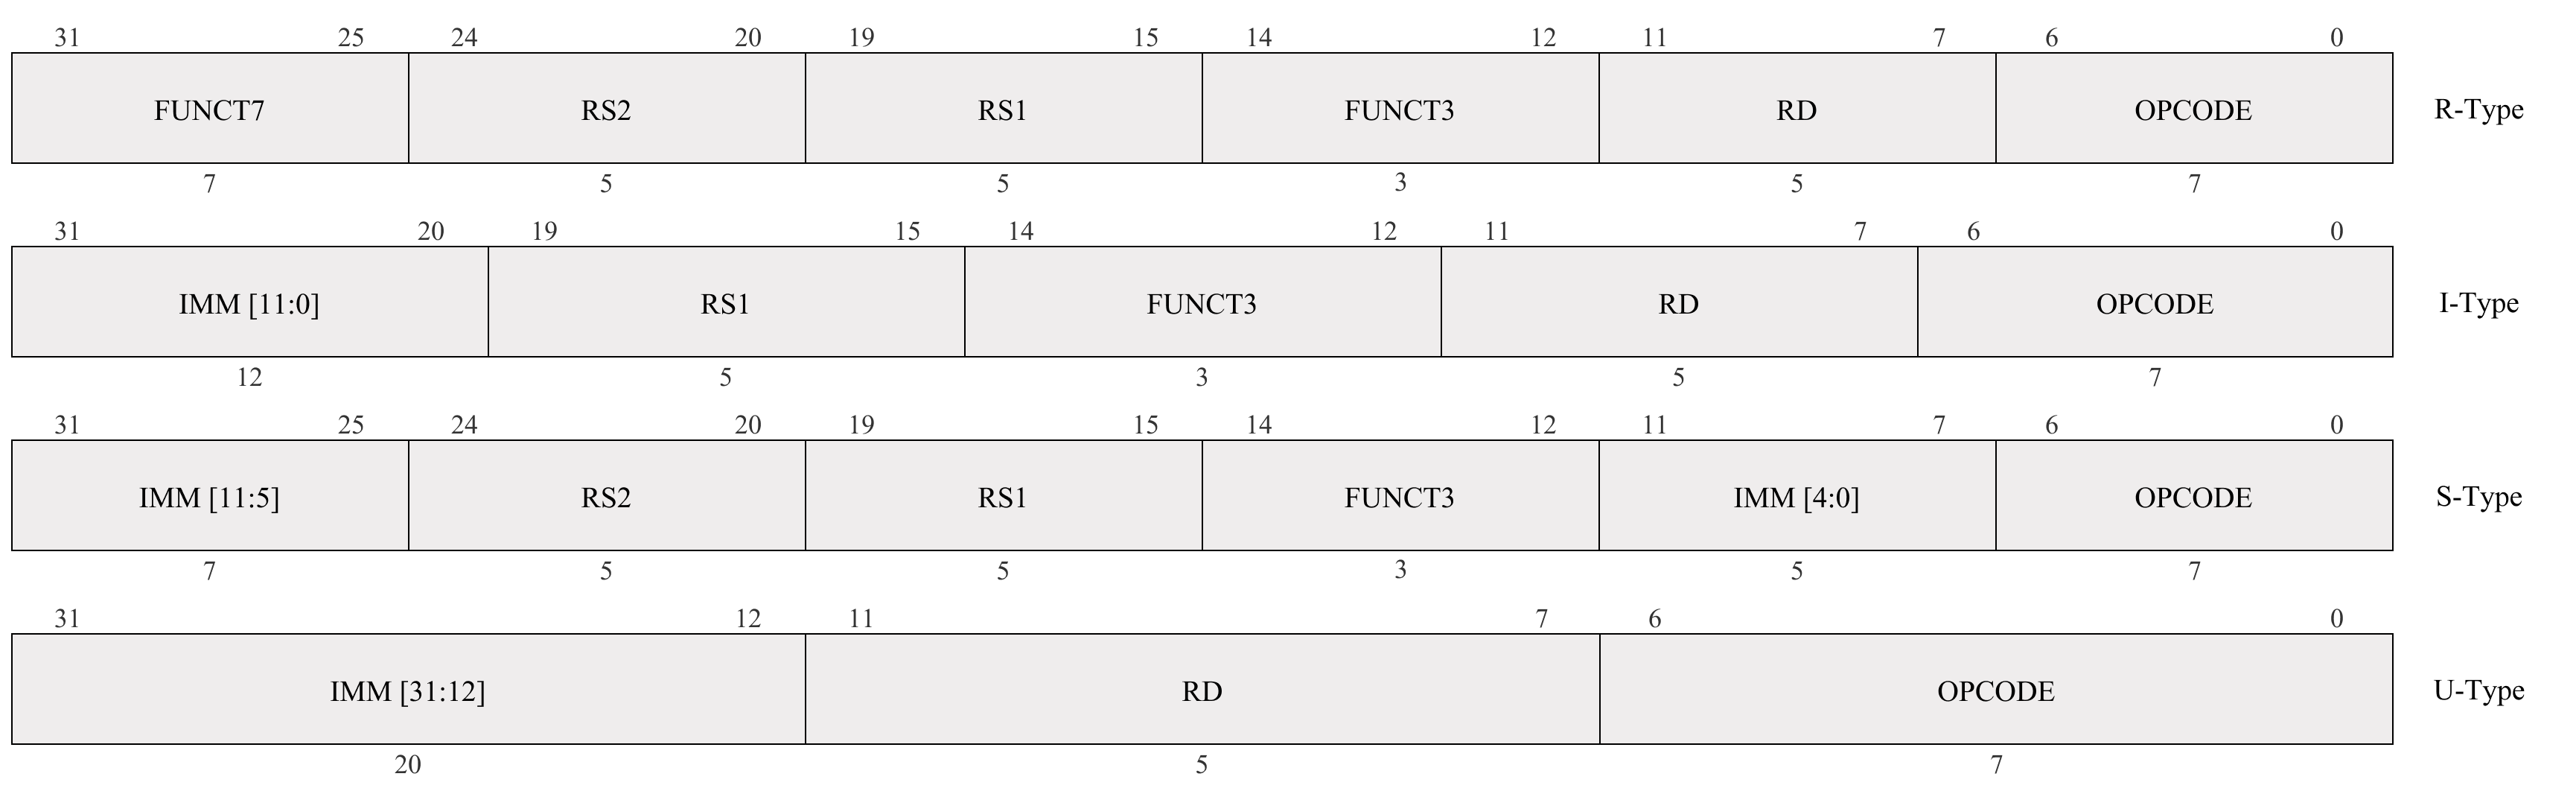
\includegraphics[width=.9\linewidth]{images/instrformats.png}}
  {\scriptsize }
  \caption{RISC-V Base Instruction Formats}
  \label{fig:instrformats}
\end{figure}

\begin{figure}[htbp]
  \centering
  \def\stackalignment{r}\stackunder{ 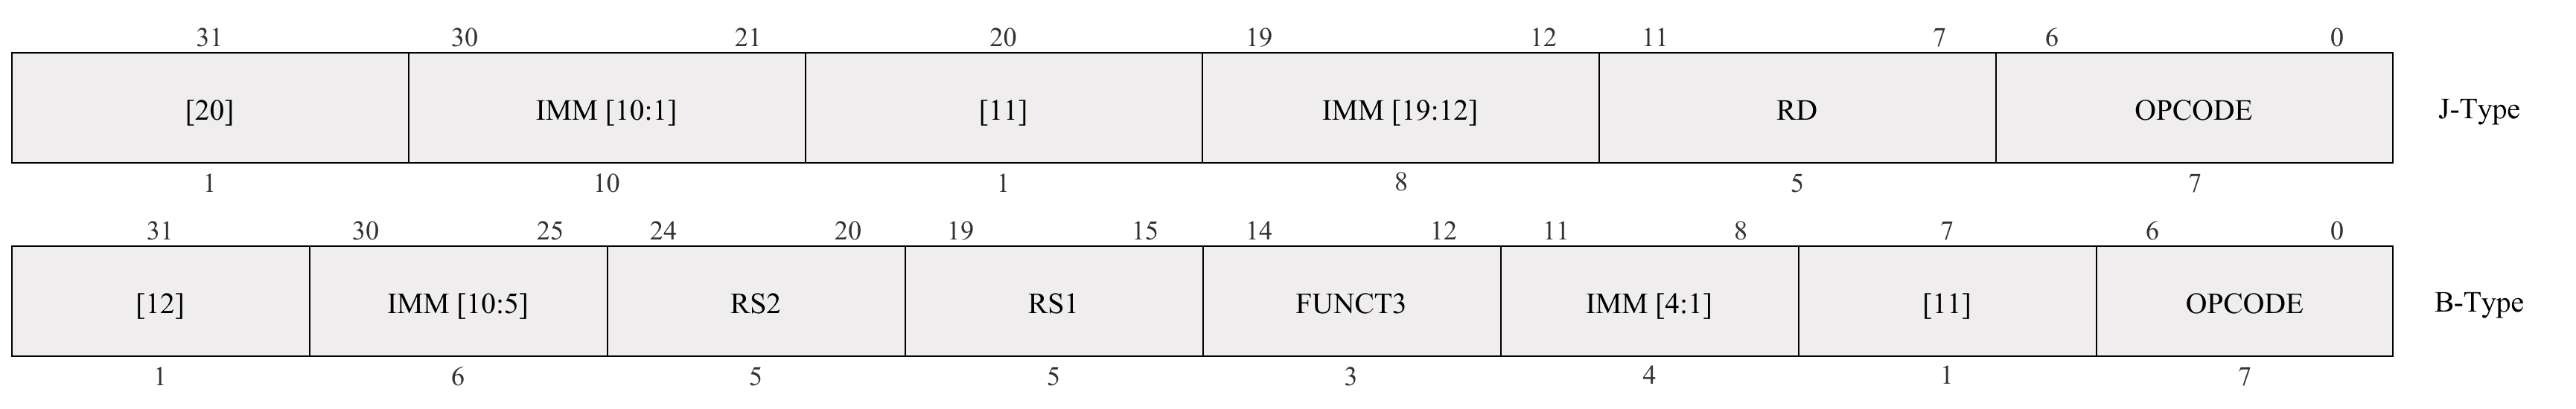
\includegraphics[width=.9\linewidth]{images/extrainstrformats.png} } %
  {\scriptsize }
  \caption{RISC-V Extra Instruction Formats}
  \label{fig:extrainstrformats}
\end{figure}

The \textit{RISC-V} ISA keeps the source (\textit{RS1} and \textit{RS2}) and
destination (\textit{RD}) registers in the same position to simplify instruction
decoding. Immediate values (\textit{IMM}) are always sign-extended and generally
stored in the most significant available bits. Lastly, \textit{FUNCT3}, \textit{FUNCT7}
and \textit{OPCODE} are used to define the operation.

\subsection{Control Transfer Instructions}
\label{subsec:riscv_controltransfer}

In this subsection, we explain \textit{RISC-V}'s control transfer instructions
which are fundamental for this project.

\textit{RV32I} defines two types of control transfer instructions: unconditional
jumps and conditional branches.

\subsubsection{Unconditional Jumps}
\label{subsubsec:riscv_unconditionalj}

\textit{RISC-V} defines two types of unconditional jumps: jump and link (\textit{JAL})
and jump and link register (\textit{JALR}).

The \textit{JAL} instruction is encoded using the \textit{J}-type format. The
immediate offset is sign-extended and added to the address of the jump
instruction (current \textit{pc}\footnote{\textit{pc} stands for program counter
and holds the address of the current instruction}) to determine the jump target
address. As a result, jumps can target a range within $\pm 1 MiB$ from their
address. Moreover, \textit{JAL} stores the address of the instruction following the
jump ($\textit{pc}+ 4$) into the destination register \textit{RD}.

The \textit{JALR} instruction is encoded using the \textit{I}-type format. The immediate
offset is sign-extended and added to the source register \textit{RS1} to
determine the jump target address (also the least-significant bit of the result is
set to $0$). Similarly to \textit{JAL}, \textit{JALR} stores the address of the
instruction following the jump ($\textit{pc}+ 4$) into the destination register
\textit{RD}.

Lastly, a plain unconditional jump is provided under the pseudo-instruction
\textit{J} and it is simply encoded as a \textit{JAL} instruction with
$\textit{RD}= x0$.

\subsubsection{Conditional Branches}
\label{subsubsec:riscv_conditionalb}

\textit{RISC-V} defines six branch instructions that compare two registers. \textit{BEQ}
and \textit{BNE} take the branch if registers \textit{RS1} and \textit{RS2} are equal
or different respectively. \textit{BLT} and \textit{BLTU} take the branch if
\textit{RS1} is less than \textit{RS2}, using signed and unsigned comparison respectively.
Lastly, \textit{BGE} and \textit{BGEU} take the branch if \textit{RS1} is
greater than or equal to \textit{RS2}, using signed and unsigned comparisons
respectively.

All conditional branch instructions are encoded using the \textit{B}-type format.
The immediate offset is sign-extended and added to the address of the branch
instruction (current \textit{pc}) to determine the branch target address. As a
result, conditional branches can target a range within $\pm 4 \textit{KiB}$ from
their address.

\subsection{Environment Calls and Breakpoints}
\label{subsec:riscv_ecalls}

\textit{RISC-V} defines two classes of \textit{SYSTEM} instructions which are
used to access system functionalities that may require privileged access. These instructions
are encoded using the \textit{I}-type format. The two classes are those that read-modify-write
Control and Status Registers, and all other potentially privileged instructions.

Control and Status Registers will be discussed later, while among the second class
of \textit{SYSTEM} instructions, we need to define \textit{ECALL} and \textit{EBREAK}.
\textit{ECALL} is used to perform a service request to the execution environment.
The Execution Environment Interface (EII) defines how parameters should be
passed. Instead, \textit{EBREAK} is used to return control to a debugging environment.

\section{RISC-V Exceptions, Traps and Interrupts}
\label{sec:riscv_eti}

In \textit{RISC-V}, exceptions are unusual conditions tied to the execution of
an instruction within the \textit{hart}\footnote{A \textit{hart} in \textit{RISC-V}
is defined as a hardware thread}, while interrupts are external asynchronous events
that may cause an unexpected control transfer within the \textit{hart}. Both exceptions
and interrupts lead to a trap, which causes a control transfer to a trap handler.

Traps in RISC-V can have four possible effects, each corresponding to how the trap
is managed:

\begin{itemize}
  \item Contained Trap: The trap is visible to software in the current execution
    environment and is handled within it. For example, in an EII that provides
    both Machine and User mode , an \textit{ECALL} made by user-mode will generally
    result in a transfer of control to a machine-mode handler within the same \textit{hart};

  \item Requested Trap: A synchronous exception explicitly requesting the
    execution environment to perform an action on behalf of the software inside
    the environment. The software may or may not resume execution on the \textit{hart}
    afterward;

  \item Invisible Trap: The execution environment handles the trap transparently,
    so the running software is unaware of it. An example is handling device
    interrupts for a different job. In this case, the software is not aware of
    the trap and the execution continues normally;

  \item Fatal Trap: This indicates a critical failure, causing the execution environment
    to terminate execution. An example is failing a virtual-memory page-protection
    check.
\end{itemize}

\begin{table}
  \centering
  \begin{tabular}{|c|c|c|c|c|}
    \hline
    \textbf{}                           & \textbf{Contained} & \textbf{Requested} & \textbf{Invisible} & \textbf{Fatal} \\
    \hhline{=====} Execution terminates & No                 & No                 & No                 & Yes            \\
    \hline
    Software is oblivious               & No                 & No                 & Yes                & Yes            \\
    \hline
    Handled by environment              & No                 & Yes                & Yes                & Yes            \\
    \hline
  \end{tabular}
  \caption{RISC-V privilege levels}
  \label{tab:traps}
\end{table}

As we will see later, traps are handled thanks to a trap vector table which is
responsible for managing the trap, deciding the outcome, and resuming the
execution when needed.

\section{RISC-V Privilege Levels}
\label{sec:riscv_privileges}

\textit{RISC-V} defines multiple privilege levels to manage access to system
resources and control execution modes. These privilege levels are designed to provide
a secure and efficient framework for managing different software components,
such as operating systems, hypervisors, and user applications.

As it's possible to see in Table \ref{tab:priv} \textit{RISC-V} implements three
different privilege levels with the following characteristics:

\begin{itemize}
  \item Machine Mode (M-mode): Machine mode is the most privileged and
    fundamental level in the \textit{RISC-V} architecture. It is the only
    required privilege level in all \textit{RISC-V} implementations and provides
    complete access to hardware resources and system configurations. It is
    responsible for configuring the hardware, setting up system resources, and
    initializing other privilege levels. Furthermore, trap handling is performed
    by M-mode;

  \item Supervisor Mode (S-mode): Supervisor mode is an optional privilege level
    designed for running operating systems or hypervisors. It offers more privileges
    than U-mode but less than M-mode. S-mode enables an operating system to
    manage resources and control hardware with enough authority while ensuring
    that user applications cannot access or alter critical system configurations;

  \item User Mode (U-mode): User mode is the least privileged level and is
    designed for running user-level applications. It restricts access to critical
    system resources, ensuring that any malicious or faulty application cannot
    compromise the overall system. U-mode's restricted environment makes it ideal
    for running user applications securely, providing a balance between
    performance and protection.
\end{itemize}

\begin{table}
  \centering
  \begin{tabular}{|c|c|c|c|}
    \hline
    \textbf{Level}  & \textbf{Encoding} & \textbf{Name}    & \textbf{Abbreviation} \\
    \hhline{====} 0 & 00                & User/Application & U                     \\
    \hline
    1               & 01                & Supervisor       & S                     \\
    \hline
    2               & 10                & Reserved         & -                     \\
    \hline
    3               & 11                & Machine          & M                     \\
    \hline
  \end{tabular}
  \caption{RISC-V privilege levels}
  \label{tab:priv}
\end{table}

\section{RISC-V General Purpose Registers}
\label{sec:riscv_reg}

The base \textit{RISC-V} ISA provides $32$ general purpose registers all $32$ bits
wide. Table \ref{tab:registers} depicts all the described registers.

Except for \textit{x0} which is hardwired to $0$ no other registers are assigned
to a specific role. However, the standard calling convention uses:
\begin{itemize}
  \item register \textit{x1}: as return address for a \textit{JAL} or \textit{JALR}
    instruction;

  \item register \textit{x5}: as an alternate link register for \textit{JAL} and
    \textit{JALR} instructions;

  \item register \textit{x2}: as the stack pointer;

  \item \textit{t}-registers: as temporary registers which are to be saved by the
    caller when needed;

  \item \textit{a}-registers: as function arguments and return values;

  \item \textit{s}-registers: as saved registers which are to be saved by the callee
    when needed.
\end{itemize}

\begin{table}
  \centering
  \begin{tabular}{|c|c|c|}
    \hline
    \textbf{Register}        & \textbf{Alias}  & \textbf{Calling Convention Description}    \\
    \hhline{===} \textit{x0} & \textit{zero}   & Hard-wired zero                            \\
    \hline
    \textit{x1}              & \textit{ra}     & Return address                             \\
    \hline
    \textit{x2}              & \textit{sp}     & Stack pointer                              \\
    \hline
    \textit{x3}              & \textit{gp}     & Global pointer                             \\
    \hline
    \textit{x4}              & \textit{tp}     & Thread pointer                             \\
    \hline
    \textit{x5}              & \textit{t0}     & Temporary register/alternate link register \\
    \hline
    \textit{x6-x7}           & \textit{t1-t2}  & Temporary registers                        \\
    \hline
    \textit{x8}              & \textit{s0/fp}  & Saved register/frame pointer               \\
    \hline
    \textit{x9}              & \textit{s1}     & Saved register                             \\
    \hline
    \textit{x10-x11}         & \textit{a0-a1}  & Function arguments/return values           \\
    \hline
    \textit{x12-x17}         & \textit{a2-a7}  & Function arguments                         \\
    \hline
    \textit{x18-x27}         & \textit{s2-s11} & Saved registers                            \\
    \hline
    \textit{x28-x32}         & \textit{t3-t6}  & Temporary registers                        \\
    \hline
  \end{tabular}
  \caption{\textit{RISC-V} General Purpose Registers}
  \label{tab:registers}
\end{table}

\section{RISC-V Control and Status Registers (CSRs)}
\label{sec:riscv_csrs}

\textit{RISC-V} defines a separate address space of $4096$ Control and Status
Registers (CSRs) associated with each \textit{hart}. CSRs are particular
registers used to control specific functions of the machine. Thanks to the \textit{ZICSR}
standard extension we can import into our ISA the following CSR-related
instructions:
\begin{itemize}
  \item \textit{CSRRW} (Atomic Read/Write CSR): atomically swaps values in the CSRs
    and integer registers. \textit{CSRRW} reads the old value of the CSR and writes
    it to the destination register (\textit{RD}). The initial value in the source
    register (\textit{RS1}) is written to the CSR. If the destination register is
    \textit{x0}, then the instruction will not read the CSR;

  \item \textit{CSRRS} (Atomic Read and Set Bits in CSR): reads the value of the
    CSR and writes it to the destination register (\textit{RD}). The initial value
    in the source register (\textit{RS1}) is treated as a bit mask that
    specifies bit positions to be set in the CSR;

  \item \textit{CSRRC} (Atomic Read and Clear Bits in CSR): reads the value of the
    CSR and writes it to the destination register (\textit{RD}). The initial value
    in the source register (\textit{RS1}) is treated as a bit mask that
    specifies bit positions to be cleared in the CSR.
\end{itemize}
All CSR instructions atomically read-modify-write a single CSR, whose specifier
is encoded in the $12$-bit \textit{CSR} field (Image \ref{fig:csrinstr} shows
the encoding of CSR instructions).

\begin{figure}[htbp]
  \centering
  \def\stackalignment{r}\stackunder{ 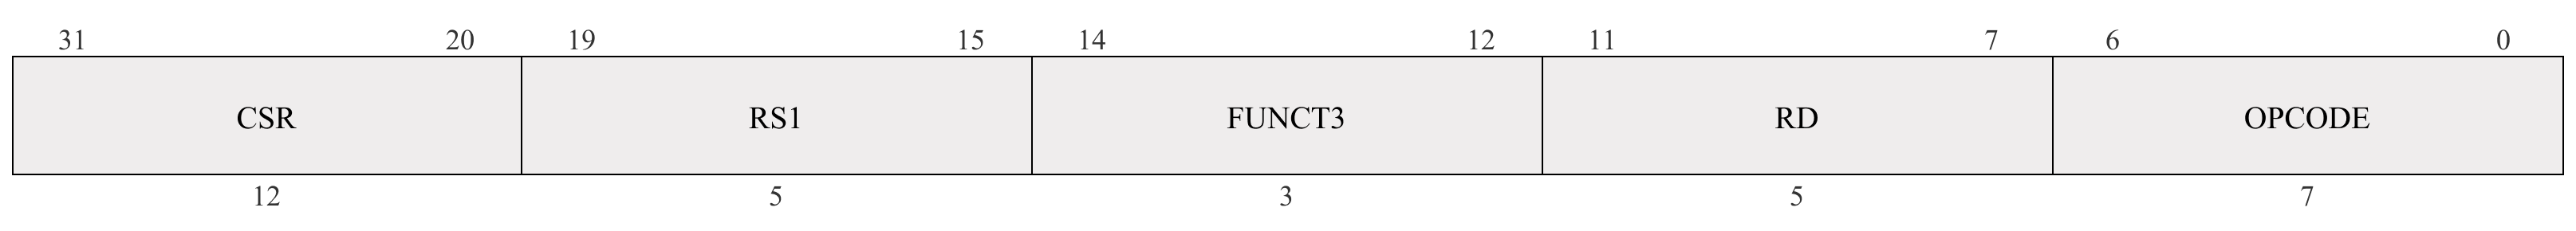
\includegraphics[width=.9\linewidth]{images/csr_instructions.png} } %
  {\scriptsize }
  \caption{Control and Status Register instructions encoding}
  \label{fig:csrinstr}
\end{figure}

Table \ref{tab:csrop} depicts whether a CSR is read or written by every
operation.

\begin{table}
  \centering
  \begin{tabular}{|c|c|c|c|c|}
    \hline
    \textbf{Instruction} & \textbf{Destination reg is x0} & \textbf{Source reg is x0} & \textbf{Reads CSR} & \textbf{Writes CSR} \\
    \hhline{=====} CSRRW & Yes                            & -                         & No                 & Yes                 \\
    \hline
    CSRRW                & No                             & -                         & Yes                & Yes                 \\
    \hline
    CSRRS/CSRRC          & -                              & Yes                       & Yes                & No                  \\
    \hline
    CSRRS/CSRRC          & -                              & No                        & Yes                & Yes                 \\
    \hline
  \end{tabular}
  \caption{CSR operation outcome}
  \label{tab:csrop}
\end{table}

Out of all the CSRs, only a few will be described in the following sections
since they will be necessary to understand the functioning of this project.

\subsection{Machine Status Register (MSTATUS) CSR}
\label{subsec:mstatus}

The \textit{mstatus} register keeps track of and controls the \textit{hart}'s current
operating state. This register will be used to manage interrupts and privilege
levels. Figure \ref{fig:mstatus} depicts a representation of the \textit{mstatus}
CSR.

\begin{figure}[htbp]
  \centering
  \def\stackalignment{r}\stackunder{ 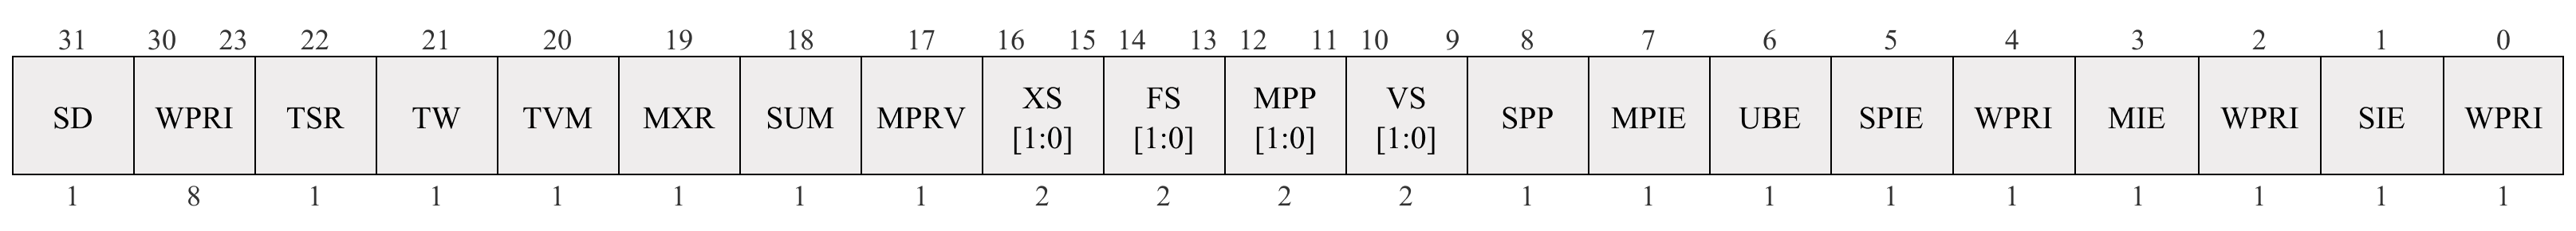
\includegraphics[width=.9\linewidth]{images/mstatus_csr.png} } %
  {\scriptsize }
  \caption{Machine Status Register (\textit{mstatus})}
  \label{fig:mstatus}
\end{figure}

Each field in \textit{mstatus} is used to control a specific function of the ISA.
Specifically, the fields are:
\begin{itemize}
  \item Global interrupt-enable bits \textit{MIE} and \textit{SIE} are used to enable
    and disable interrupts for M-mode and S-mode respectively. When a \textit{hart}
    is executing in privilege mode \textit{x}, interrupts are globally enabled when
    $\textit{xIE}= 1$ and globally disabled when $\textit{xIE}= 0$. Interrupts
    for privilege modes \textit{w}, where $\textit{w}< \textit{x}$ are always
    globally disabled regardless of any \textit{wIE} bit set. Interrupts for
    privilege modes \textit{y}, where $\textit{y}> \textit{x}$ are always
    globally enabled regardless of any \textit{yIE} bit set;

  \item \textit{SPIE}, \textit{MPIE}, \textit{SPP}, and \textit{MPP} are used
    when managing a trap. \textit{SPIE} and \textit{MPIE} hold the previous interrupt
    enable bit for S-mode and M-mode respectively. \textit{SPP} and \textit{MPP}
    hold the previous privilege level for S-mode and M-mode respectively. These bits
    are used to track the status of the machine prior to the trap and are necessary
    to correctly restore the context before returning from a trap;

  \item The modify privilege bit \textit{MPRV} modifies the effective privilege
    mode. When $\textit{MPRV}= 0$ loads and store behave normally while, if
    $\textit{MPRV}= 1$ load and store memory addresses are translated and
    protected;

  \item The make executable readable \textit{MXR} bit modifies the privilege
    with which loads access virtual memory. When $\textit{MXR}=0$, only loads
    from pages marked readable will succeed. When $\textit{MXR}=1$, loads from
    pages marked either readable or executable will succeed;

  \item The supervisor user memory access \textit{SUM} bit modifies the
    privilege with which S-mode loads and stores access virtual memory. When $\textit
    {SUM}=0$, S-mode memory accesses to pages that are accessible by U-mode will
    fault. When $\textit{SUM}=1$, these accesses are permitted;

  \item The trap virtual memory \textit{TVM} bit supports intercepting
    supervisor virtual-memory management operations. When $\textit{TVM}=1$,
    attempts to read or write the \textit{satp} CSR while executing in S-mode will
    raise an illegal-instruction exception. When $\textit{TVM}=0$, these operations
    are permitted in S-mode;

  \item The timeout wait \textit{TW} bit supports intercepting the WFI
    instruction. When $\textit{TW}=0$, the WFI instruction may execute in lower
    privilege modes. When $\textit{TW}=1$, then if WFI is executed in any less-privileged
    mode and it does not complete within a time limit, the WFI instruction causes
    an illegal-instruction exception;

  \item The trap sret \textit{TSR} bit supports intercepting the supervisor
    exception return instruction, \textit{SRET}. When $\textit{TSR}=1$, attempts
    to execute \textit{SRET} while executing in S-mode will raise an illegal-instruction
    exception. When $\textit{TSR}=0$, this operation is permitted in S-mode;

  \item The \textit{FS}, \textit{VS}, and the \textit{XS} fields are used to
    reduce the cost of context save and restore by setting and tracking the
    current state of the floating-point unit and any other user-mode extensions
    respectively.
\end{itemize}

\subsection{Machine Exception Program Counter (MEPC) CSR}
\label{subsec:mepc}

The \textit{mepc} register is used, when a trap is taken in M-mode, to store the
address of the instruction that was interrupted or that encountered the
exception. Figure \ref{fig:mepc} depicts a representation of \textit{mepc}.

\begin{figure}[htbp]
  \centering
  \def\stackalignment{r}\stackunder{ 
\includegraphics[width=.9\linewidth]{images/mepc_csr.png} } %
  {\scriptsize }
  \caption{Machine Exception Program Counter (\textit{mepc})}
  \label{fig:mepc}
\end{figure}

\subsection{Machine Cause Register (MCAUSE) CSR}
\label{subsec:mcause}

The \textit{mcause} register is used, when a trap is taken in M-mode, to store the
code that indicates the event that caused the trap. All the possible codes can
be seen in Table \ref{tab:causes}. Figure \ref{fig:mcause} depicts a representation
of \textit{mcause}.

\begin{figure}[htbp]
  \centering
  \def\stackalignment{r}\stackunder{ 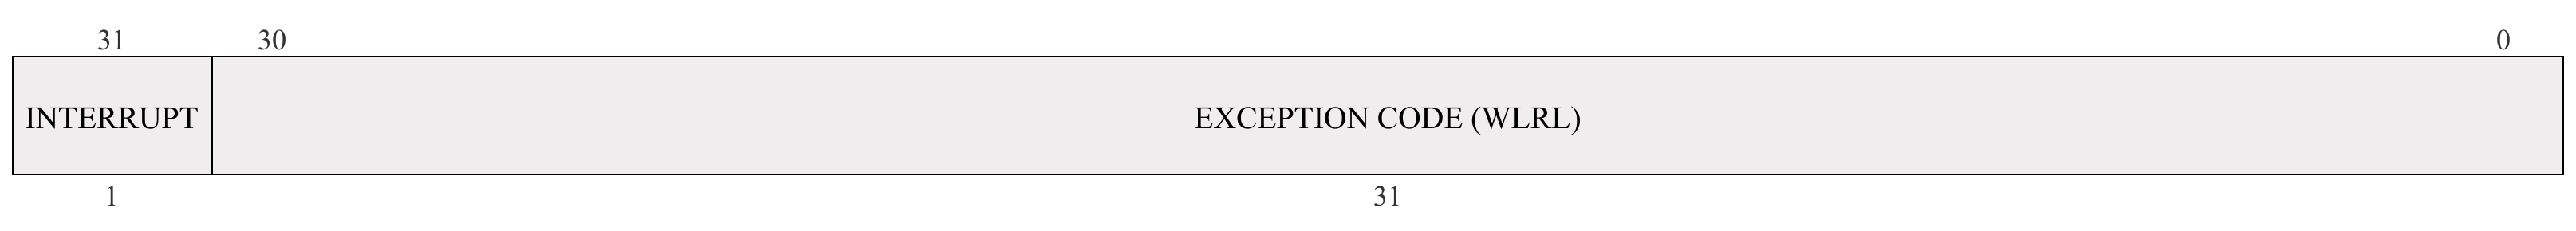
\includegraphics[width=.9\linewidth]{images/mcause_csr.png} } %
  {\scriptsize }
  \caption{Machine Cause Register (\textit{mcause})}
  \label{fig:mcause}
\end{figure}

\begin{table}
  \centering
  \begin{tabular}{|c|c|c|}
    \hline
    \textbf{Interrupt} & \textbf{Code} & \textbf{Description}           \\
    \hhline{===} 1     & 0             & User software interrupt        \\
    \hline
    1                  & 1             & Supervisor software interrupt  \\
    \hline
    1                  & 2             & Reserved                       \\
    \hline
    1                  & 3             & Machine software interrupt     \\
    \hline
    1                  & 4             & User timer interrupt           \\
    \hline
    1                  & 5             & Supervisor timer interrupt     \\
    \hline
    1                  & 6             & Reserved                       \\
    \hline
    1                  & 7             & Machine timer interrupt        \\
    \hline
    1                  & 8             & User external interrupt        \\
    \hline
    1                  & 9             & Supervisor external interrupt  \\
    \hline
    1                  & 10            & Reserved                       \\
    \hline
    1                  & 11            & Machine external interrupt     \\
    \hline
    1                  & 12            & Reserved                       \\
    \hline
    1                  & 13            & Counter-overflow interrupt     \\
    \hline
    1                  & 14-15         & Reserved                       \\
    \hline
    1                  & $\geq 16$     & Designated for platform use    \\
    \hhline{===} 0     & 0             & Instruction address misaligned \\
    \hline
    0                  & 1             & Instruction access fault       \\
    \hline
    0                  & 2             & Illegal instruction            \\
    \hline
    0                  & 3             & Breakpoint                     \\
    \hline
    0                  & 4             & Load address misaligned        \\
    \hline
    0                  & 5             & Load access fault              \\
    \hline
    0                  & 6             & Store/AMO address misaligned   \\
    \hline
    0                  & 7             & Store/AMO access fault         \\
    \hline
    0                  & 8             & Environment call from U-mode   \\
    \hline
    0                  & 9             & Environment call from S-mode   \\
    \hline
    0                  & 10            & Reserved                       \\
    \hline
    0                  & 11            & Environment call from M-mode   \\
    \hline
    0                  & 12            & Instruction page fault         \\
    \hline
    0                  & 13            & Load page fault                \\
    \hline
    0                  & 14            & Reserved                       \\
    \hline
    0                  & 15            & Store/AMO page fault           \\
    \hline
    0                  & 16-17         & Reserved                       \\
    \hline
    0                  & 18            & Software check                 \\
    \hline
    0                  & 19            & Hardware check                 \\
    \hline
    0                  & 20-23         & Reserved                       \\
    \hline
    0                  & 24-31         & Designated for custom use      \\
    \hline
    0                  & 32-47         & Reserved                       \\
    \hline
    0                  & 48-63         & Designated for custom use      \\
    \hline
    0                  & $\geq 64$     & Designated for custom use      \\
    \hline
  \end{tabular}
  \caption{Interrupts and Exception causes}
  \label{tab:causes}
\end{table}

\subsection{Machine Trap Value Register (MTVAL) CSR}
\label{subsec:mtval}

The \textit{mtval} register is used, when a trap is taken in M-mode, to store
exception-specific information to assist software in handling the trap. Figure \ref{fig:mcause}
depicts a representation of \textit{mtval}.

\begin{figure}[htbp]
  \centering
  \def\stackalignment{r}\stackunder{ 
\includegraphics[width=.9\linewidth]{images/mtval_csr.png} } %
  {\scriptsize }
  \caption{Machine Trap Value Register (\textit{mtval})}
  \label{fig:mtval}
\end{figure}

\subsection{Machine Trap-Vector Base-Address Register (MTVEC) CSR}
\label{subsec:mtvec}

The \textit{mtvec} register is used to store the address that holds the trap vector
configuration. Figure \ref{fig:mtvec} depicts a representation of \textit{mtvec}.
The \textit{MODE} field can be set according to Table \ref{tab:mode}. If we set
the \textit{MODE} to vectored, all asynchronous interrupts will set the program
counter to the base address encoded in \textit{mtvec} plus $4$ times the cause of
the interrupt (causes can be seen in Table \ref{tab:causes}). With \textit{MODE}
set to direct instead, all traps set the program counter to the base address.

\begin{figure}[htbp]
  \centering
  \def\stackalignment{r}\stackunder{ 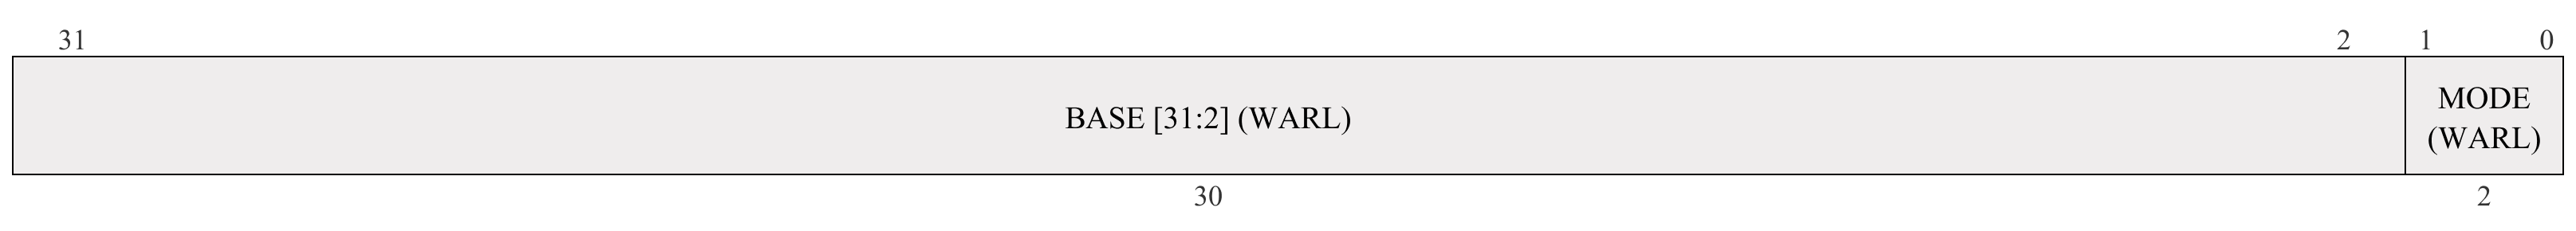
\includegraphics[width=.9\linewidth]{images/mtvec_csr.png} } %
  {\scriptsize }
  \caption{Machine Trap-Vector Base-Address Register (\textit{mtvec})}
  \label{fig:mtvec}
\end{figure}

\begin{table}
  \centering
  \begin{tabular}{|c|c|c|}
    \hline
    \textbf{Value}   & \textbf{Name} & \textbf{Description}                                                      \\
    \hhline{===} $0$ & Direct        & All traps set $\textit{pc}= \textit{BASE}$                                \\
    \hline
    $1$              & Vectored      & Asynchronous interrupts set $\textit{pc}= \textit{BASE}+4*\textit{cause}$ \\
    \hline
    $\geq 2$         & -             & Reserved                                                                  \\
    \hline
  \end{tabular}
  \caption{Encoding of \textit{MODE} for \textit{mtvec} register}
  \label{tab:mode}
\end{table}

\section{RISC-V Physical Memory Protection (PMP)}
\label{sec:riscv_pmp}

\textit{RISC-V} provides an optional Physical Memory Protection (PMP) unit that
allows to configure access privileges (read, write, and execute) for each
physical memory region. The PMP ensures secure processing and helps to contain faults.

PMP checks are applied at all accesses in S or U mode. Optionally, PMP checks may
additionally apply to M-mode accesses, in which case the PMP registers
themselves are locked, so that even M-mode software cannot change them until the
hart is reset. Each PMP check results either in a violation which is trapped at
the processor or in a granted permission.

\subsection{PMP CSRs}
\label{subsec:riscv_pmpcsr}

Each PMP entry is described by an 8-bit configuration register (\textit{pmpXcfg})
and one $32$-bit address register (\textit{pmpaddrX}). Sixteen CSRs, \textit{pmpcfg0-pmpcfg15},
hold the configurations \textit{pmp0cfg-pmp63cfg} for the 64 PMP entries (as shown
in Figure \ref{fig:pmpcfgs}). Each PMP address (\textit{pmpaddr0-pmpaddr63})
encodes bits $33$-$2$ of a $34$-bit physical address as shown in Figure
\ref{fig:pmpaddr}.

Each PMP configuration register (Figure \ref{fig:pmpconf}) contains:
\begin{itemize}
  \item R-bit: when set allows read access;

  \item W-bit: when set allows write access;

  \item X-bit: when set allows instruction execution;

  \item A-bits: used to set address matching mode (better explained in subsection
    \ref{subsec:pmpaddressmatching});

  \item L-bit: when set the configuration is locked, meaning that it can't be modified
    without a system reset.
\end{itemize}

\begin{figure}[htbp]
  \centering
  \def\stackalignment{r}\stackunder{ 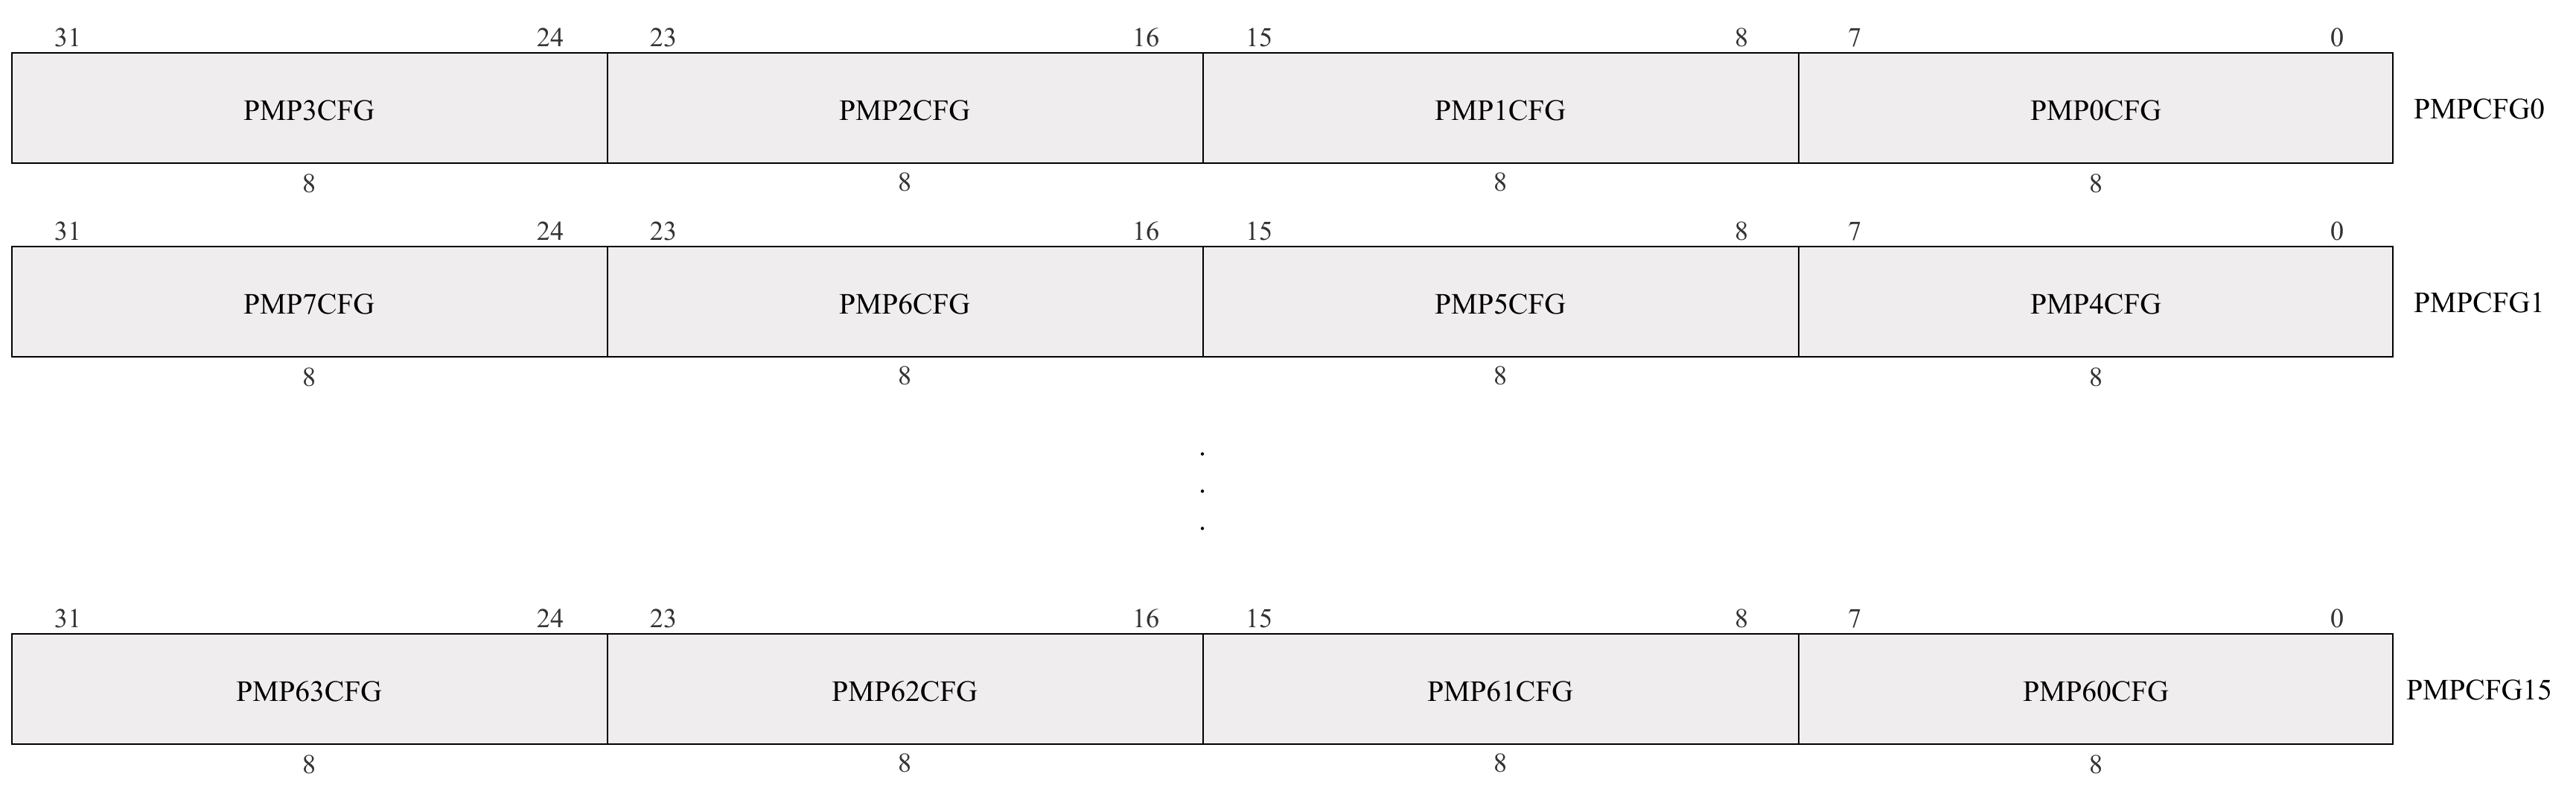
\includegraphics[width=.9\linewidth]{images/pmpcfgs_csr.png}}
  {\scriptsize Source: \href{https://drive.google.com/file/d/17GeetSnT5wW3xNuAHI95-SI1gPGd5sJ_/view}{\textit{RISC-V} Privileged Manual}}
  \caption{PMP Configuration CSR (\textit{pmpcfg0-pmpcfg15})}
  \label{fig:pmpcfgs}
\end{figure}

\begin{figure}[htbp]
  \centering
  \def\stackalignment{r}\stackunder{ 
\includegraphics[width=.9\linewidth]{images/pmpaddress_csr.png} } %
  {\scriptsize }
  \caption{PMP Address CSR (\textit{pmpaddr})}
  \label{fig:pmpaddr}
\end{figure}

\begin{figure}[htbp]
  \centering
  \def\stackalignment{r}\stackunder{ 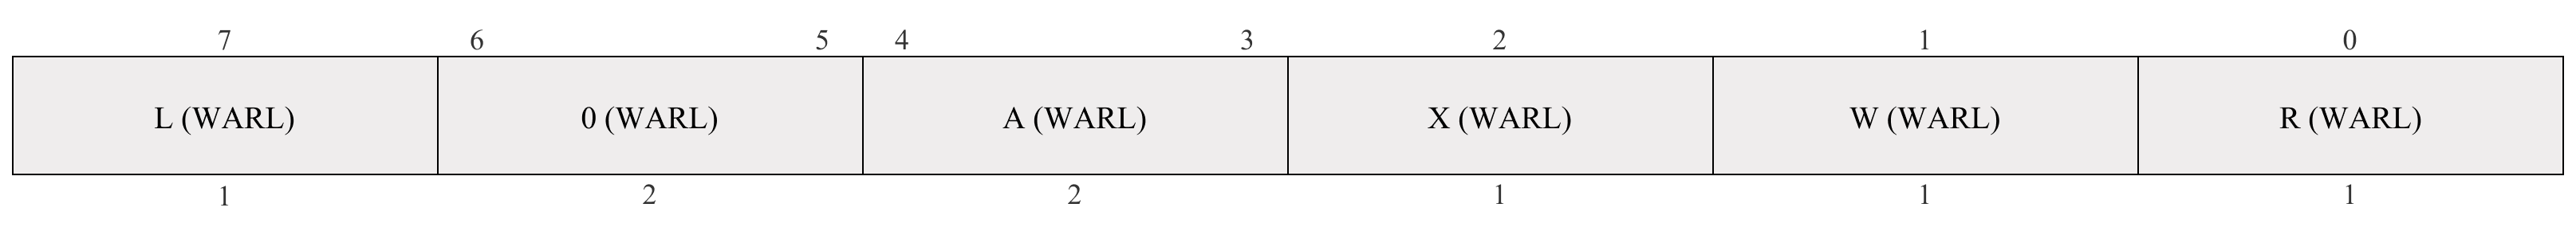
\includegraphics[width=.9\linewidth]{images/pmpconf_csr.png} } %
  {\scriptsize }
  \caption{PMP Configuration Register Format}
  \label{fig:pmpconf}
\end{figure}

\subsection{PMP Address Matching}
\label{subsec:pmpaddressmatching}

The A field in a PMP entry's configuration register encodes the address-matching
mode of the associated PMP address register (encoding shown in Table \ref{tab:addressmatching}).

\begin{table}
  \centering
  \begin{tabular}{|c|c|c|}
    \hline
    \textbf{A}       & \textbf{Name} & \textbf{Description}                  \\
    \hhline {===} 00 & OFF           & Null region (disabled)                \\
    \hline
    01               & TOR           & Top of range                          \\
    \hline
    10               & NA4           & Naturally aligned four-byte region    \\
    \hline
    11               & NAPOT         & Naturally aligned power-of-two region \\
    \hline
  \end{tabular}
  \caption{Encoding of A field in PMP Configuration Register}
  \label{tab:addressmatching}
\end{table}

When $A=0$, this PMP entry is disabled and matches no addresses. Two other address-matching
modes are supported:
\begin{itemize}
  \item Naturally aligned power-of-$2$ regions (NAPOT): NAPOT ranges make use of
    the low-order bits of the associated address register to encode the size of
    the range. This includes the special case of naturally aligned four-byte regions
    (NA4);

  \item Top boundary of an arbitrary range (TOR): If TOR is selected, the associated
    address register forms the top of the address range, and the preceding PMP
    address register forms the bottom of the address range. Note that, if the
    first PMP address is configured as TOR the lower boundary is considered to
    be \textit{0x0}.
\end{itemize}

\subsection{PMP Matching Logic}
\label{subsec:matchinglogic}

PMP entries are statically prioritized. The lowest-numbered PMP entry that matches
any byte of an access determines whether that access succeeds or fails. The
matching PMP entry must match all bytes of an access, or the access fails,
irrespective of the L, R, W, and X bits. For example, if a PMP entry is configured
to match the four-byte range \textit{0xC-0xF}, then an $8$-byte access to the range
\textit{0x8-0xF} will fail, assuming that such PMP entry is the highest-priority
entry that matches those addresses.

If a PMP entry matches all bytes of an access, then the L, R, W, and X bits determine
whether the access succeeds or fails. If the L bit is clear and the privilege
mode of the access is M, the access succeeds. Otherwise, if the L bit is set or the
privilege mode of the access is S or U, then the access succeeds only if the R, W,
or X bit corresponding to the access type is set.

If no PMP entry matches an S-mode or U-mode access, but at least one PMP entry is
implemented, the access fails. Failed accesses generate a load, store, or instruction
access exception.